\section{Monolayer}

Throughout our work, $\hbar = 1$.

\n

Graphene is an allotrope of graphite and consists of a hexagonal lattice of carbon atoms linked in $sp^2$ hybridization with distance $a$, where $3$ electrons from carbon form $\s$ bonds and the last electron is located on a $\pi$ orbital and is the only one that matters for the electronic properties of the material.

\n

Our convention is zig-zag in horizontal direction and arm-chair in vertical direction.

\begin{figure}[H]
\centering
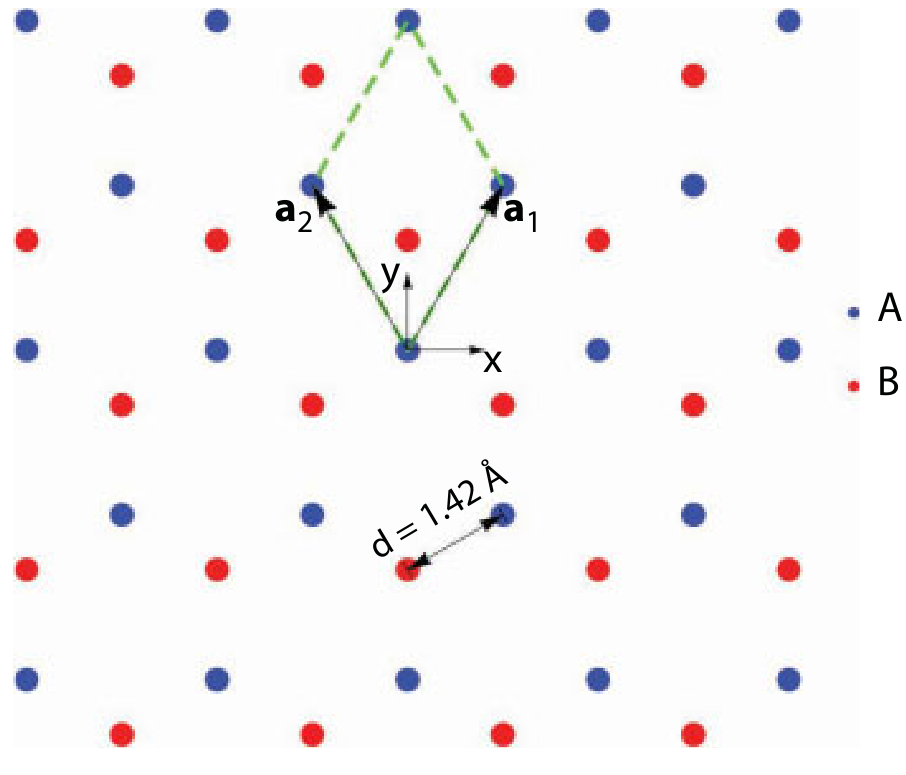
\includegraphics[width=0.4\linewidth]{fig/graphene-lattice_vectors2.png}
\label{fig:graphene-lattice_vectors}
\caption{\textcolor{red}{Graphene lattice vectors. Taken from \cite{handbook2019}}}
\end{figure}

The lattice vectors are $\vb{a}_1 = a \qty(\frac{1}{2}, \frac{\sqrt{3}}{2})$, $\vb{a}_2 = a \qty(-\frac{1}{2}, \frac{\sqrt{3}}{2})$. The unit cell area is $ A_1 = \abs{\a_1 \times \a_2} = \frac{\sqrt{3}}{2} a^2 $.

The Brillouin zone is
\begin{figure}[H]
\centering
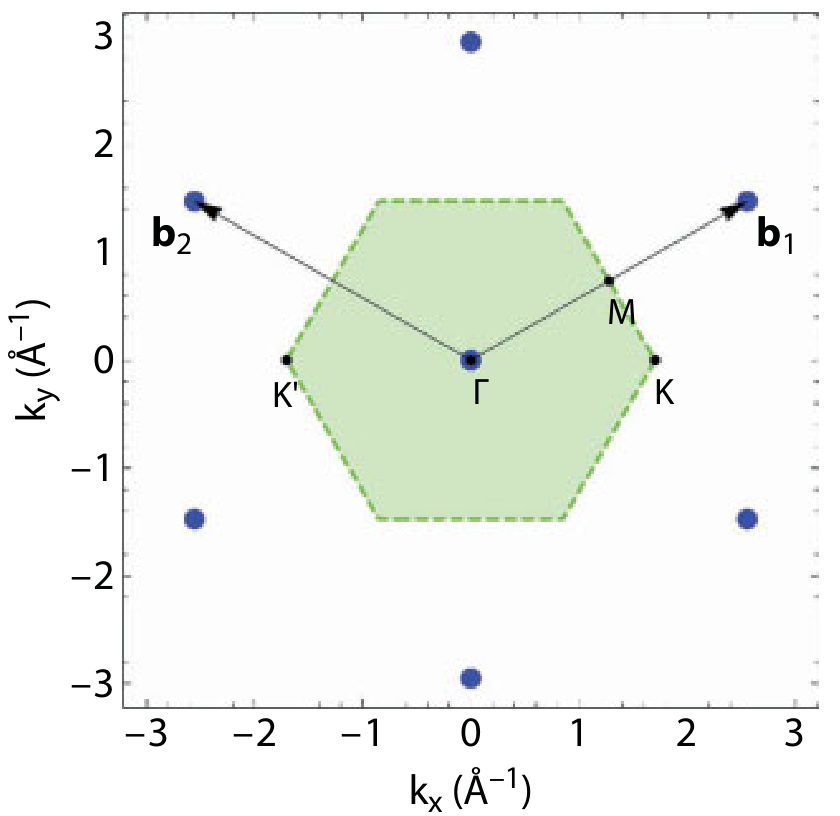
\includegraphics[width=0.3\linewidth]{fig/brillouin-zone-monolayer.png}
\caption{\textcolor{red}{Graphene Brillouin Zone. Taken from \cite{handbook2019}}}
\label{fig:brillouin-zone-monolayer}
\end{figure}

Using the convention $\a_3 = \vu{z}$, the momentum lattice vectors are
\begin{equation} \label{eq:monolayer-bvecs}
\b_1 = \frac{2\pi}{A_1} \a_2 \times \a_3 = \frac{4\pi}{\sqrt{3} a } \qty(\frac{\sqrt{3}}{2}, \frac{1}{2}), \quad
\b_2 = \frac{2\pi}{A_1} \a_3 \times \a_1 = \frac{4\pi}{\sqrt{3} a } \qty(-\frac{\sqrt{3}}{2}, \frac{1}{2}).
\end{equation}

The two main Dirac points are defined as
\begin{equation} \label{eq:monolayer-dirac-points}
\K = \frac{4\pi}{3a} (1, 0) , \quad \K' = -\K.
\end{equation}



We write a tight-binding hamiltonian with only nearest-neighbor hopping
\begin{equation} \label{eq:monolayer-tight-binding}
H = -t \sum_{\R} c^\d_B(\R) \qty(c_A(\R) + c_A(\R-\a_1) + c_A(\R-\a_2)) + \hc,
\end{equation}
where the $\R$ sum runs through all the associated Bravais triangular lattice. Applying the Fourier transforms
\begin{equation} \label{eq:monolayer-fourier}
c_{\alpha}^\d(\R) = \frac{1}{\sqrt{N}} \sum_{\k \in \text{BZ}} e^{-i \k \vdot \r_i} c_A^\d(\k),
\end{equation}
we get
\begin{equation} \label{eq:monolayer-tight-binding2}
H = \sum_{\k}
\begin{pmatrix}
c_A^\d(\k) & c_B^\d(\k)
\end{pmatrix}
\begin{pmatrix}
0 & -t f(\k) \\
-t f^*(\k) & 0
\end{pmatrix}
\begin{pmatrix}
c_A^\d(\k) \\ c_B^\d(\k)
\end{pmatrix},
\end{equation}
with
\begin{equation} \label{eq:monolayer-fk}
f(\k) = \sum_{\nu} e^{i \k \vdot \bm{\delta}_\nu} =
e^{idk_y} + 2 e^{-\frac{idk_y}{2}} \cos(\frac{\sqrt{3}}{2} dk_x),
\end{equation}
where $\bm{\delta}_1 = (\a_1 + \a_2)/3 = d (0, 1)$, $\bm{\delta}_2 = (-2\a_1 + \a_2)/3 = d(-\frac{\sqrt{3}}{2}, -\frac{1}{2})$, $\bm{\delta}_3 = (\a_1 - 2\a_2)/3 = d (\frac{\sqrt{3}}{2}, -\frac{1}{2})$ are the vectors that connect to the three nearest neighboring sites, and $d = a/\sqrt{3}$.

\n

The eigenenergies of hamiltonian \ref{eq:monolayer-tight-binding2} are $E_\pm(\k) = \pm t \abs{f(\k)}$. Notice that the points $\K$ and $\K'=-\K$ are roots of $f$, i.e., $f(\pm\K) = 0$. These are the so-called Dirac points, around which the dispersion relation are approximately linear $E(\K + \q) = v_F \abs{\q} + O(\abs{\q}/\abs{\K})^2$.


%%%%%-----
%%%%% Referências bibliográficas
%%%%%-----
%%%\addcontentsline{toc}{chapter}{\bibname}
%%%%\bibliographystyle{abntex2-num}
%%%\bibliography{citations}
%%%\bibliographystyle{ieeetr}
